\documentclass{article}
\usepackage[utf8]{inputenc}
\usepackage{listings}
\usepackage{svg}
\usepackage{hyperref}
\usepackage{minted}
\usepackage{caption}
\usepackage{amsmath}
\usepackage{subcaption}
\setminted{fontsize=\footnotesize}
\lstset{frame=tb,   language=Python,   aboveskip=3mm,   belowskip=3mm,   showstringspaces=false,   columns=flexible,   basicstyle={\small\ttfamily},   numbers=none,   numberstyle=\tiny\color{gray},   keywordstyle=\color{blue},   commentstyle=\color{dkgreen},   stringstyle=\color{mauve},   breaklines=true,   breakatwhitespace=true,   tabsize=3 }

\title{Digital Signal Processing\\Assignment 3\\Fluid Pressure Sensing}
\author{2324362M - Connor MacLean\\2324421J - Alban Joseph}
\date{December 2020}

\begin{document}
\maketitle
Declaration of Originality and Submission Information.\\
I affirm that this submission is my own / the groups original work in accordance with the University of Glasgow Regulations and the School of Engineering Requirements.
\section{Introduction}
In various applications, it is desirable to monitor the pressure of a liquid in a tank. This can be done using a pressure sensor, however noise often needs to be removed, e.g.:
\begin{enumerate}
  \item Noise exists when monitoring the pressure of a fuel tank on a moving vehicle - the vibrations from driving would effect the signal measured. Hence, in order to determine the correct pressure, the signal could be passed through a filter to remove any noise.
  \item Industrial control systems often rely on accurate pressure measurements to monitor and optimise industrial processes. The process of adding or removing liquid from a tank can result in noise being introduced into the measurement system (movement of water causes changes in pressure). The raw signal from a pressure sensor will contain this noise on top of the low frequency signal we desire to measure. In industrial environments, accurate measurements of pressure often allows for the flow rate to be calculated and further adjustments to be made.
\begin{figure}[H]
    \centering
    \includesvg[scale=0.25]{figure1}
    \caption{Control System Data Flow Diagram}
    \label{fig:controlSys}
\end{figure}
To optimise the controllers response the high frequency noise must be removed from from our signal.
\end{enumerate}
In this experiment, we will take raw data from a pressure sensor and filter out any noise to achieve an accurate pressure reading. The experimental set up for real time data acquisition is displayed below in Figure 2a.
\begin{figure}[H]
\centering
\begin{subfigure}{.5\textwidth}
  \centering
  \includesvg[scale=0.25]{figure3}
  \caption{}
  \label{fig:a}
\end{subfigure}%
\begin{subfigure}{.5\textwidth}
  \centering
  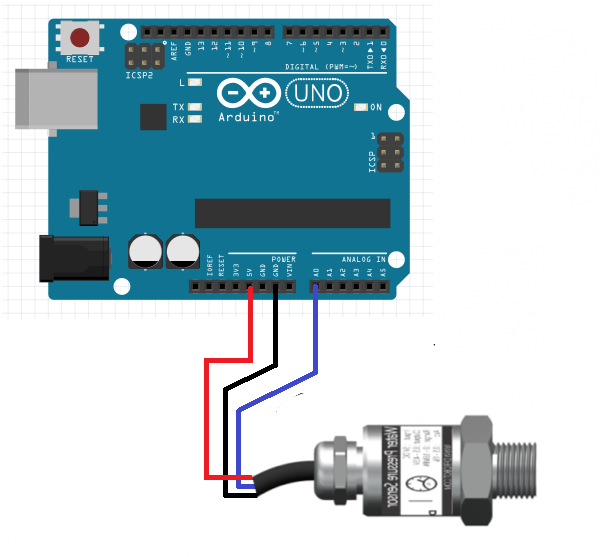
\includegraphics[scale=0.45]{pressureCircuit}
  \caption{}
  \label{fig:b}
\end{subfigure}
\caption{Experimental Set Up}
\label{fig:setUp}
\end{figure}
An Arduino Uno was used to sample data and the sensor was connected to the Arduino as shown in Figure 2b. The raw signal captured by the Arduino was sent into a python file to be filtered.
By disturbing the water and applying pressure to the outside of the tank we can create noise. A video detailing the experimental setup, and the results from the experiment, is available at \url{https://youtu.be/qxcsjcHZ_OI}
 
\section{Sampling Rate Verification}
A class was created in the `timer.py' to check the sampling rate of the system:
\begin{lstlisting}
import time

class Timer:
    def __init__(self):
        self._start_time = None
        self.sampleCount = 0

    def start(self):
        #Start a new timer
        self._start_time = time.perf_counter()

    def reset(self):
        #Stop the timer, reset the counter, start the timer.
        self._start_time = None
        self.sampleCount = 0
        self._start_time = time.perf_counter()

    def time(self):
        #returns time elapsed
        elapsed_time = time.perf_counter() - self._start_time
        return elapsed_time
    
    def frequency(self):
        #determines frequency from time elapsed
        frequency = 1/(time.perf_counter() - self._start_time)
        return frequency
\end{lstlisting}
Several functions were created in this class for different purposes.
\begin{itemize}
  \item start(): starts a timer using the perf\_counter() function.
  \begin{itemize}
  \item perf\_counter() returns a value (in fractional seconds) of a performance counter, i.e. a clock with the highest available resolution to measure a short duration.
  \end{itemize}  
  \item reset(): stops the counter, resets all variables and starts a new timer again.
  \item time(): returns the time passed since the timer was started.
  \item frequency(): measures the time elapsed (since the timer started) and returns the frequency associated with this time interval.
\end{itemize}
The sampling rate of the acquisition was checked by running it for 10 seconds.\newline
The sampling rate should be 100Hz, so over 10 seconds, 1000 samples should be captured. In the main section of the code, a timer, `t', was started and the following code was placed in the `callBack' function; hence, it was executed every time the data was to be plotted:
\lstset{language=Python}
\begin{lstlisting}
t.sampleCount += 1 #increments number of samples counted
if t.time() >= 10: #if 10 seconds have passed
    print(t.sampleCount, ``= number of samples taken in 10 seconds'')
    t.reset() #resets the timer and sample count to 0
\end{lstlisting}
Objects of this timer class contain a variable used to count the number of samples captured - `sampleCount'. This variable is incremented every time a new data point is sampled. If 10 seconds have passed, then the number of samples captured is printed to the screen.
\newline
\begin{figure}[H]
    \centering
    \includesvg[scale=0.15]{rippleCounter}
    \caption{Sampling Rate over 10 seconds}
    \label{fig:tenSecs}
\end{figure}
\newline 
The code was run for slightly longer than one minute to improve the accuracy of the results. From Figure \ref{fig:tenSecs}, it is clear that a small inconsistency existed in the sampling: an extra one or two samples was being counted every ten seconds. This may be due to jitter. Jitter describes the timing errors in the sampling operation (often caused by clock disturbances). To identify jitter the above code was altered to the following:
\lstset{language=Python}
\begin{lstlisting}
print(t.frequency(), ``Hz'') #prints the sampling frequency
t.reset() #clock is reset
\end{lstlisting}
Every time data is captured a timer is reset. The `frequency' function measures the time between each sample and returns the frequency from this time interval, i.e. the sampling frequency.
\newline
\begin{figure}[H]
    \centering
    \includesvg[scale=0.25]{sampleFrequency}
    \caption{Sampling Rate between consecutive points}
    \label{fig:sampleF}
\end{figure}
\newline 
The sampling frequency varied from 80Hz to 120Hz, approximately . However, it was noted that occasionally the sampling frequency was measured to be over 5000Hz. This was considered to be jitter. Some heuristics could be put into place to ensure wrongly acquired data would not be plotted by:
\lstset{language=Python}
\begin{lstlisting}
def callBack(data):
    if t.frequency() < 1000: #if sampling frequency is less than 1000Hz
        #code for plotting data here
    t.reset() #resets timer
\end{lstlisting}
If the frequency measured between two consecutive points exceed 1000Hz then the data is not plotted. This was not included in our final implementation as 1 or 2 extra data points did not drastically effect the function of the system.

\section{Frequency Response}
\subsection{Desired Transfer Function}
The raw signal data relevant to the system is very low frequency. The volume of liquid in the tank will not be changing drastically so anything above 1Hz is deemed to be unimportant and therefore removable. Therefore the ideal frequency response for this system is a low pass Filter with cut off frequency at 1Hz.
\begin{figure}[H]
    \centering
    \includesvg[scale=0.75]{lowpass}
    \caption{Ideal Low Pass Filter}
    \label{fig:lowpass}
\end{figure}

\subsection{Butterworth Vs Chebyshev}
The Butterworth filter provides minimal ripple in the pass band and beyond cut off in comparison to the Chebyshev filter. This comes at the expense of a lower roll of rate. For this application the role of rate is of less importance so the Butterworth filter was chosen. To produce a lowpass response a high level design command was used.
\lstset{language=Python}
\begin{lstlisting}
samplingRate = 100 #sampling rate: 100Hz
f1 = 1
sos = signal.butter(5,2*f1/samplingRate, output = 'sos')
#coeffs should filter everything except DC
#frequency normalised to Nyquist
\end{lstlisting}
The Discrete frequency normalised to Nyquist is given to the function. The sos coefficients returned are for 5th order IIR filter. 
\newline
The SOS coefficients generated by the high level function `signal.butter' are formatted as follows:
 \[
   sos =
\begin{bmatrix}
b_0 & b_1 & b_2 & a_0 & a_1 & a_2\\
b_0 & b_1 & b_2 & a_0 & a_1 & a_2\\
b_0 & b_1 & b_2 & a_0 & a_1 & a_2
\end{bmatrix} \approx
\begin{bmatrix}
2.8e-08 & 5.5e-08 & 2.8e-08 & 1 & -9.4e-01 & 0\\
1 & 2 & 1 & 1 & -1.9 & 9.0e-01\\
1 & 1 & 0 & 1 & -1.9 & 9.6e-01
\end{bmatrix}
\]
Where each row contains coefficients for a 2nd order IIR Filter.

\section{Filter Class}
\subsection{2nd Order Filter}
The `IIR2filter' class contains a function which implements a 2nd order IIR filter. The coefficients a0, a1, a2, b0, b1, b2 (gain blocks in Figure \ref{fig:dataFlow}) are given as the arguments for the constructor. These coefficients are stored and two buffers are initialised. The IIR filter operation is outline below in both code and a data flow diagram.
\begin{figure}[H]
    \centering
    \includesvg[scale=0.25]{figure4}
    \caption{Direct Form II 2nd Order IIR Data Flow Diagram}
    \label{fig:dataFlow}
\end{figure}
This is a direct form II implementation, it uses two accumulators and two delay steps to implement the following transfer function:
\[H(z) = \frac{b_0+b_1z^-^1+b_2z^-^2}{a_0+a_1z^-^1+a_2z^-^2}\]
A 2nd order IIR filter, represented by the above equation, was programmed:
\begin{lstlisting}
def filter(self, x): #need to create two accumulators
    acc_input = self.a0*x - self.buffer1*self.a1 - self.buffer2*self.a2 #accumulator for IIR part
    acc_output = acc_input*self.b0 + self.buffer1*self.b1 + self.buffer2*self.b2 #FIR accumulator
    self.buffer2 = self.buffer1
    self.buffer1 = acc_input
    return acc_output
\end{lstlisting}
This `filter' method takes an incoming data value as the argument and uses the coefficients (stored in the constructor) to return a filtered value.

\subsection{Chain of 2nd Order Filters}
Cascading second order IIR filters allows for the overall quality of the filtered signal to be improved whilst ensuring it remains relatively easy to design.
\begin{figure}[H]
    \centering
    \includesvg[scale=0.25]{figure5}
    \caption{Cascaded IIR Filter Dataflow Diagram}
    \label{fig:dataFlow}
\end{figure}
A second class was defined to implement this. The sos array produced from the scipy.signal.butter function was taken as the constructor argument.
\begin{lstlisting}
def __init__(self, sos): #constructor function
        self.filt = [] #list of instances of IIR2Filter
        for x in range(len(sos)): #repeat for all rows in sos array
            self.filt.append(IIR2filter(sos[x][0], sos[x][1], sos[x][2], sos[x][3], sos[x][4], sos[x][5]))
            #creates IIR2Filter instance with sos array
            #and stores instance in list
\end{lstlisting}
self.filt is a list of 2nd order IIR filters. The `filter' method (in this class) takes an incoming data point, sends it through the stored IIR filters and returns the output:
\begin{lstlisting}
def filter(self, x): 
    inP = x #store incoming data point in inP
    for i in range(len(self.filt)): #repeat for all filters
        outP = self.filt[i].filter(inP) #output of filter[i]
        inP = outP #IIR filter output becomes input of next filter
    return outP
\end{lstlisting}
The incoming data point is stored in a variable inP, where inP is the input to the upcoming IIR filter. The output from the IIR filter is calculated and stored in outP. inP = outP sets the output calculated to be the input of the following IIR filter. This is repeated until there are no more IIR filters in the self.filt list. The final value for outP is returned.

\subsection{Testing the Cascading IIR Filters}
To ensure the IIRFilter filter function sends incoming data through a chain of 2nd order IIR2Filters, a test was created.
\begin{lstlisting}
def response(sos): #plots frequency and impulse response from sos coeffs
    filt = IIRfilter(sos) #creates chain of 2nd order filters

    x=np.zeros(100,dtype=complex) #creating impulse response
    x[10]=1

    y=np.zeros(100,dtype=complex)
    for i in range(len(x)):
        y[i]= filt.filter(x[i]) #result of impulse response stored in y
        
    plt.figure(1)
    plt.plot(y)
    #plots impulse response
    plt.figure(2)
    plt.plot(np.linspace(0,1,len(y)), abs(np.fft.fft(y)))
    #plots transfer function
    plt.show()
\end{lstlisting}
This function takes the sos array as its argument and creates a chain of 2nd order filters. An impulse function is created and sent through the chain to determine the impulse response. The frequency response is calculated using an FFT. The impulse response and the frequency response of the IIRFilter filter are then plotted, as shown in Figure \ref{fig:reponse}:
\begin{figure}[H]
\centering
\begin{subfigure}{.5\textwidth}
  \centering
  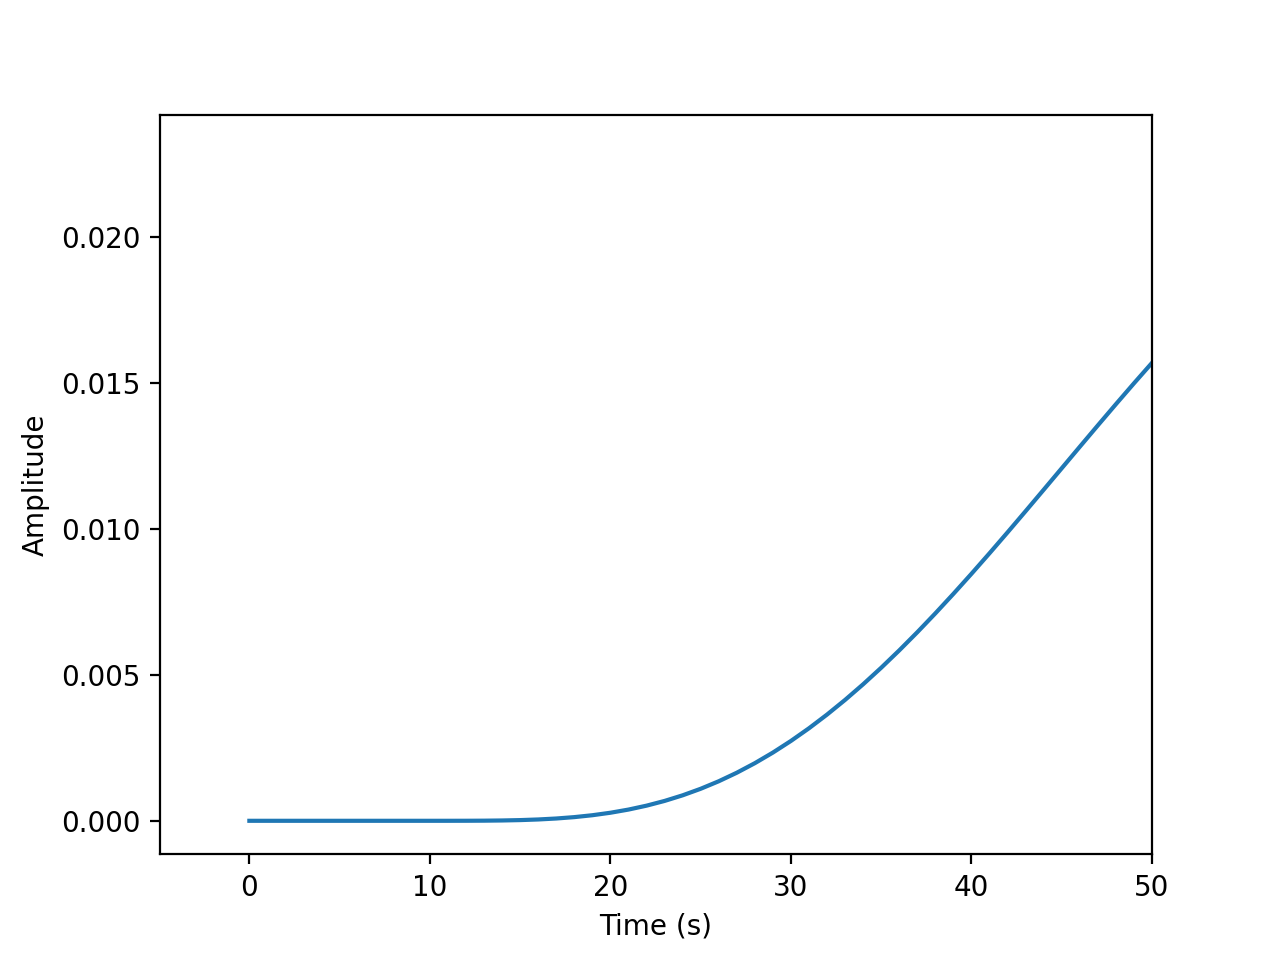
\includegraphics[scale=0.4]{iResponse}
  \caption{Impulse Response}
  \label{fig:a}
\end{subfigure}%
\begin{subfigure}{.5\textwidth}
  \centering
  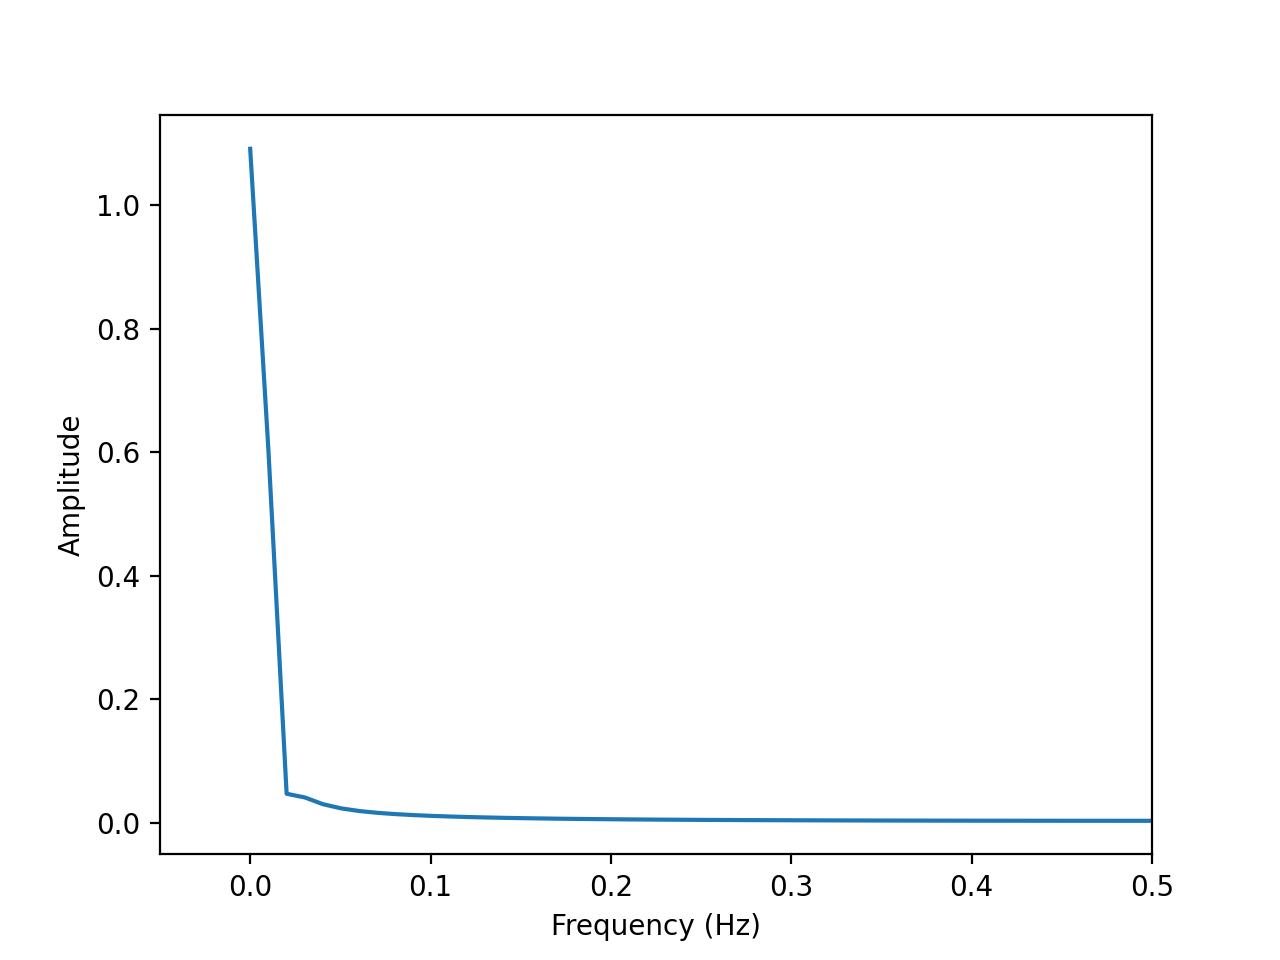
\includegraphics[scale=0.4]{fResponse}
  \caption{Frequency Response}
  \label{fig:b}
\end{subfigure}
\caption{5th Order Low Pass Filter Response}
\label{fig:reponse}
\end{figure}
This method to determine the filter response was favourable as it ensures the IIR filter was constructed correctly.

\section{Results}
The QPlanningPlot class (from the example on the github repo) was used to plot, and hence compare, the raw data with the filtered signal - as seen in Figure \ref{fig:filtered}. The high frequency noise present in the signal was completely removed by the low pass IIR filter. 
\begin{figure}[H]
    \centering
    \includesvg[scale=0.13]{filterResults}
    \caption{Unfiltered Vs Filtered Signal}
    \label{fig:filtered}
\end{figure}
The low frequency signal, i.e. the desired pressure reading, was maintained sufficiently. The filtered signal follows the original data well, although a small time delay exists. IIR filters have nonlinear phase response so as the number of filters cascaded increases, the phase delay also increases. This filter, therefore, is well suited for pressure sensing a fuel tank (and other applications monitoring signal amplitudes). However, this system would not be appropriate for industrial control systems, where phase delay is an important factor.\newline
This filter uses minimal memory space and little computing power ($\approx$24 calculations per sample) to adequately remove high frequency noise above 1Hz; therefore, for our purposes, the overall filtering operation has been successful. 


\pagebreak

\section{Appendix}
\subsection{realtime\_iir\_main.py}
\inputminted{python}{realtime_iir_main.py}

\pagebreak
\subsection{IIR\_Filter.py}
\inputminted{python}{IIR_filter.py}

\pagebreak
\subsection{timer.py}
\inputminted{python}{timer.py}

\pagebreak
\subsection{realtimescope.py}
\inputminted{python}{realtimescope.py}
\end{document}